\chapter{半导体中载流子的统计分布}
在一定的温度下,如果没有其他外界作用,半导体中的导电电子和空穴是依靠电子的热激发作用而产生的,电子从不断热振动的晶格中获得一定的能量,就可能从低能量的量子态跃迁到高能量的量子态,例如,电子从价带跃迁到导带,形成导带电子和价带空穴。除了这种本征激发的方式,通过杂质电离亦可以引入导带电子和价带空穴。这些我们已经很熟悉了,但与此同时,还有一种相反的过程,即电子当然也可以从高能量的量子态跃迁到低能量的量子态,并向晶格放出一定能量,这将使电子与空穴复合而减少,这一过程称为\uwave{载流子的复合}(Carrier Recombination),这与先前\uwave{载流子的产生}(Carrier Generation)是两个相反的过程,在一定温度下,这两个相反的过程将建立动态平衡,称为\uwave{热平衡状态}。这时,半导体中的电子浓度和空穴浓度都将保持一个稳定的数值,这种热平衡状态下的电子和空穴称为\uwave{热平衡载流子}。

实践表明,半导体的导电性强烈的随温度而变化,实际上,这种变化主要是由于半导体载流子浓度随温度变化而造成的。因此,我们很有必要先探究载流子浓度随温度变化的规律,这也就是本章的中心问题,即所谓载流子的统计分布。为此,我们需要两方面的知识
\begin{enumerate}
    \item 电子可以存在的量子态如何分布。
    \item 电子在其可以存在的量子态上如何分布。
\end{enumerate}
前者将以状态密度描述,后者将以费米--狄拉克分布或玻尔兹曼分布描述。

\section{状态密度}

\subsection{状态密度的定义}
在半导体的导带和价带中,有很多能级的存在。但相邻能级的间隔很小,约为$10^{-23}$\si{eV}的数量级,因此,可以认为能级是准连续的。故可以用状态密度描述各个能值处状态数的疏密。
\begin{BoxDefinition}[状态密度]
    定义\uwave{状态密度}(Density of States),为单位能量间隔的量子态的数目
    \begin{Equation}
        g(E)=\dv{Z}{E}
    \end{Equation}
\end{BoxDefinition}

暂且,先让我们放下状态密度,而是先研究一下状态本身是如何分布于$\vb*{k}$空间的。

我们知道,受限于晶体边界的限制,事实上$\vb*{k}$只能取一系列的分立值
\begin{Align}[12pt]
    k_x&=\frac{2\pi n_x}{L}&(n_x&=0,\pm 1,\pm 2,\cdots)\\
    k_y&=\frac{2\pi n_y}{L}&(n_y&=0,\pm 1,\pm 2,\cdots)\\
    k_z&=\frac{2\pi n_z}{L}&(n_z&=0,\pm 1,\pm 2,\cdots)
\end{Align}
其中$n_x,n_y,n_z$是整数,而$L$是晶体的线度,因此
\begin{Equation}
    V=L^3
\end{Equation}
就是晶体的体积。显然在$\vb*{k}$空间,每一组整数$(n_x,n_y,n_z)$都将对应波矢$\vb*{k}$的一个可行的取值$(k_x,k_y,k_z)$,或者说,对应$\vb*{k}$空间中的一个点$(k_x,k_y,k_z)$,而$\vb*{k}$空间中的每个可取的点就代表要给可行的量子态。由于任意代表点的坐标,沿三条坐标轴的方向均为$2\pi/L$的整数倍,所以代表点在$\vb*{k}$空间中是均匀分布的,每一个代表点都可以具有$8\pi^3/L^3=8\pi^3/V$立方体积。

因此,在$\vb*{k}$空间中电子的能量状态密度是$V/8\pi^3$,由于每个能量上可以存在两个自旋方向相反的电子,所以,在$\vb*{k}$空间中电子的状态密度就是$V/4\pi^3$,是均匀的。但需要注意的是,此处求出的$V/4\pi^3$的“状态密度”与\xref{def:状态密度}中$g(E)$的“状态密度”是两回事,\empx{前者是单位体积的状态,后者是单位能量区间的状态}。不过,这两者间是有联系的,因为,能值在$\vb*{k}$空间中表现为等能面的形式,该等能面上的量子态都具有相应能值,换言之,单位能量区间的状态数实际上就是$\vb*{k}$空间中一个等能面薄层中的状态数。这也就是下面我们求解$g(E)$的思路。

\subsection{状态密度的计算}\setpeq{状态密度的计算}

下面我们来推导半导体能带极值附近的状态密度,简单起见,姑且考虑导带底,并假设导带底位于$\vb*{k}=\vb*{0}$且等能面为球面的情况,根据\xref{subsec:有效质量的引入}中的相关公式,能量--波矢关系为
\begin{Equation}&[1]
    E(\vb*{k})=E_\text{c}+\frac{\hbar^2k^2}{2\mne}
\end{Equation}
在$\vb*{k}$空间中,以$\abs{\vb*{k}}$为半径作一球面,它就是能量为$E(\vb*{k})$的等能面,而要计算$E$与$E+\dd{E}$间的量子态数,就相当于计算半径$\abs{\vb*{k}}$至$\abs{\vb*{k}+\dd{\vb*{k}}}$的球壳间的量子态数,而这两个球壳间的体积是$4\pi k^2\dd{k}$,而$\vb*{k}$空间中量子态密度是$V/4\pi^3$,故$E$至$E+\dd{E}$间的量子态数$\dd{Z}$为
\begin{Equation}&[2]
    \dd{Z}=\frac{V}{4\pi^3}\times 4\pi k^2\dd{k}=\frac{V}{\pi^2}k^2\dd{k}
\end{Equation}
而由\xrefpeq{1}可以解得
\begin{Equation}&[3]
    k^2=\frac{2\mne(E-E_\text{c})}{\hbar^2}
\end{Equation}
即
\begin{Equation}&[4]
    k=\frac{(2\mne)^{1/2}(E-E_\text{c})^{1/2}}{\hbar}
\end{Equation}
就\xrefpeq{4}求微分
\begin{Equation}&[5]
    \dd{k}=\frac{(2\mne)^{1/2}(E-E_\text{c})^{-1/2}}{2\hbar}\dd{E}
\end{Equation}
这样一来,将\xrefpeq{3}和\xrefpeq{5}代入\xrefpeq{2}
\begin{Equation}
    \dd{Z}=\frac{V}{2\pi^2}\frac{(2\mne)^{3/2}}{\hbar^3}(E-E_\text{c})^{1/2}\dd{E}
\end{Equation}
而根据\fancyref{def:状态密度}
\begin{Equation}
    g_\text{c}(E)=\dv{Z}{E}=\frac{V}{2\pi^2}\frac{(2\mne)^{3/2}}{\hbar^3}(E-E_\text{c})^{1/2}
\end{Equation}
这就表明,导带底附近的状态密度,随电子能量的增加以平方根关系增大。

\begin{Figure}[状态密度函数]
    \includegraphics[scale=0.85]{build/Chapter03A_01.fig.pdf}
\end{Figure}

而对于实际的半导体硅和锗而言,情况要比上述讨论的复杂很多,主要问题在于硅和锗的导带等能面并不是简单的球面,而是若干中心$\vb*{k}\neq\vb*{0}$对称分布的旋转椭球面,换言之,我们有两个麻烦,其一是等能面发生了变形,由球面变为了旋转椭球面,其二是导带底不只是一个状态,对于硅是$6$个,对于锗是$4$个\footnote{虽然锗有$8$个沿$\<1 1 1>$对称分布的旋转椭球面,但每个只有一半在布里渊区内,故实际只计为$4$个。},所幸的是,这两个麻烦都可以通过$\mne$重新表述解决。

\begin{BoxFormula}[导带底的状态密度]
    硅和锗在导带底的状态密度为
    \begin{Equation}
        g_\text{c}(E)=\frac{V}{2\pi^2}\frac{(2\mne)^{3/2}}{\hbar^3}(E-E_\text{c})^{1/2}
    \end{Equation}
    其中$\mne$为
    \begin{Equation}
        \mne=m_\text{dn}=s^{2/3}(m_lm_t^2)^{1/3}
    \end{Equation}
    其中$m_\text{dn}$称为导带底电子状态密度的有效质量,而$s$是对称状态的数目。
\end{BoxFormula}

需要说明的是,我们其实不必区分“有效质量”和“状态密度有效质量”的提法,因为对于硅和锗的导带电子而言,其实原本也就没有什么有效质量$\mne$的提法,只有横向有效质量$m_t$和纵向有效质量$m_l$的提法,故这里$m_t,m_l$给出的$m_\text{dn}$其实就可以视为对硅和锗$\mne$的定义。

实际上,价带顶的情况和导带底的情况是相似的,价带顶主要起作用的是极值重合的重空穴和轻空穴,如\xref{tab:硅的价带结构}所示,价带顶同样有等能面变形和存在多个极值的问题,因此价带空穴质量$\mpe$也不是简单常数,同样需用重空穴有效质量$(m_\text{p})_\text{h}$和轻空穴有效质量$(m_\text{p})_\text{l}$重表述。
\begin{BoxFormula}[价带顶的状态密度]*
    硅和锗在价带顶的状态密度为
    \begin{Equation}
        g_\text{v}(E)=\frac{V}{2\pi^2}\frac{(2\mpe)^{3/2}}{\hbar^3}(E_\text{v}-E)^{1/2}
    \end{Equation}
    其中$\mne$为
    \begin{Equation}
        \mpe=m_\text{dp}=\qty[(m_\text{p})_\text{l}^{3/2}+(m_\text{p})_\text{h}^{3/2}]^{2/3}
    \end{Equation}
    其中$m_\text{dp}$称为价带顶空穴状态密度的有效质量。
\end{BoxFormula}
在\xref{tab:半导体的状态密度有效质量}中,结合\xref{tab:硅和锗的载流子有效质量}以及硅$s=6$和锗$s=4$,列出了硅和锗等的$\mne$和$\mpe$
\begin{Table}[半导体的状态密度有效质量]{c|cccc|ccc|c}
    <
    \mrx<c>{3}{半导体材料}&\mc{4}(c|){电子}&\mc{3}(c|){空穴}&\mrx<c>{2}{比值}\\
    &纵向&横向&对称状态&有效质量&重&轻&有效质量&\\
    &$m_l$&$m_t$&$s$&$\mne$&$(m_\text{p})_\text{h}$&$(m_\text{p})_\text{l}$&$\mpe$&$\mne/\mpe$\\
    >
    硅&$0.98m_0$&$0.19m_0$&$6$&$1.06m_0$&$0.53m_0$&$0.16m_0$&$0.59m_0$&$0.59$\\
    锗&$1.64m_0$&$0.08m_0$&$4$&$0.56m_0$&$0.28m_0$&$0.044m_0$&$0.29m_0$&$0.52$\\
    砷化镓&--&--&$1$&$0.063m_0$&$0.50m_0$&$0.076m_0$&$0.52m_0$&$8.25$\\
    锑化铟&--&--&$1$&$0.012m_0$&$0.44m_0$&$0.016m_0$&$0.44m_0$&$36.7$\\
\end{Table}
在\xref{fig:状态密度函数}中,以红线和蓝线分别绘制了价带顶状态密度$g_\text{v}(E)$和导带底状态密度$g_\text{c}(E)$的曲线图像,由此可以看出,价带中能量越低,状态密度越大,导带中能量越高,状态密度越大。
\section{费米分布与玻尔兹曼分布}
在\xref{sec:状态密度}中,我们已经通过状态密度$g(E)$弄清了电子的量子态是如何分布的了,但是,并不是每一个电子可能存在的量子态都有电子存在,所以说,我们还需要找到一个电子关于能量的分布函数。事实上,尽管就单一电子而言,它所具有的能量时大时小经常变化,但是,电子按能量大小的分布具有统计规律性,这就是说,\empx{电子在不同能量上的概率密度分布是一定的}。

\subsection{费米分布}

量子统计理论指出,具有泡利不相容特性的费米子遵从费米分布,而电子作为一种费米子,其随能量$E$的概率密度分布$f(E)$也满足费米分布,这对于导带和价带(甚至禁带,只不过就算电子在禁带范围内有很高的概率密度,也没有允许电子存在的量子态)都是适用的,但是按照我们的习惯,导带讨论电子,价带讨论空穴,所以在价带中我们往往需要的是空穴的概率密度分布,空穴是电子不存在的情况,因此,空穴的统计分布其实就可以用$1-f(E)$表述。\goodbreak
\begin{BoxFormula}[费米分布]
    电子的概率密度分布遵从\uwave{费米分布}(Fermi Statistics)
    \begin{Equation}&[1]
        f(E)=\frac{1}{1+\exp(E-E_\text{F}/\kB T)}
    \end{Equation}
    空穴的概率密度分布相应遵从
    \begin{Equation}&[2]
        1-f(E)=\frac{1}{1+\exp(E_\text{F}-E/\kB T)}
    \end{Equation}
\end{BoxFormula}

在\fancyref{fml:费米分布}中的$E_\text{F}$是一个很重要的参数,称为\uwave{费米能级}(Fermi Level),它并不是一个真正的能级,只是一个具有能量量纲的参数,与温度、半导体材料、半导体的杂质类型和含量、能量零点的选取等因素有关。费米能级$E_\text{F}$作为费米分布$f(E)$的参数,具有分界线的意义,如\xref{fig:电子的统计分布}所示,\empx{费米能级是费米分布的半概率密度点},即有$f(E_\text{F})=1/2$成立。

更具体的说,电子的费米分布是这样以费米能级为界的
\begin{itemize}
    \item 在费米能级$E_\text{F}$以下,电子有较大概率出现,当$E<E_\text{F}$时有$f(E)>1/2$。
    \item 在费米能级$E_\text{F}$以上,电子有较小概率出现,当$E>E_\text{F}$时有$f(E)<1/2$。
\end{itemize}
而由\xref{fig:电子的统计分布},我们亦可以注意到温度对费米分布的影响,温度越低,费米分布的曲线在费米能级$E_\text{F}$处由$1.0$至$0.0$的跃变就越陡峭,事实上,温度为绝对零度时,此时,费米分布将转化为一个阶跃函数,换言之,电子将会完全分布在费米能级以内,严格的以最低能级填充。

而这里还有一个问题,费米能级$E_\text{F}$在哪里?事实是,\empx{费米能级通常会落在禁带中},即
\begin{Equation}
    E_\text{v}<E_\text{F}<E_\text{c}
\end{Equation}
直观上想这也是合理的,价带上有很多电子,导带上几乎没有什么电子。

\subsection{玻尔兹曼分布}
玻尔兹曼分布并不是全新的东西,它其实只不过是一定条件下对费米分布的近似。

\begin{BoxFormula}[玻尔兹曼分布]
    电子的概率密度分布在$E-E_\text{F}\gg\kB T$时遵从\uwave{玻尔兹曼分布}(Boltzmann Statistics)
    \begin{Equation}
        f(E)=\exp(\frac{E_\text{F}-E}{\kB T})
    \end{Equation}
    空穴的概率密度分布在$E-E_\text{F}\ll\kB T$时遵从
    \begin{Equation}
        1-f(E)=\exp(\frac{E-E_\text{F}}{\kB T})
    \end{Equation}
\end{BoxFormula}

\begin{Proof}
    根据\fancyref{fml:费米分布}的\xrefpeq[费米分布]{1},若$E-E_\text{F}\gg\kB T$
    \begin{Equation}*
        f(E)=\frac{1}{1+\exp(E-E_\text{F}/\kB T)}=\frac{1}{\exp(E-E_\text{F}/\kB T)}=
        \exp(\frac{E_\text{F}-E}{\kB T})
    \end{Equation}
    根据\fancyref{fml:费米分布}的\xrefpeq[费米分布]{2},若$E_\text{F}-E\gg\kB T$
    \begin{Equation}*
        1-f(E)=\frac{1}{1+\exp(E_\text{F}-E/\kB T)}=\frac{1}{\exp(E_\text{F}-E/\kB T)}=
        \exp(\frac{E-E_\text{F}}{\kB T})
    \end{Equation}
    由此可见,玻尔兹曼分布实质就是对费米分布作$1+\e^x=\e^x$近似的结果。
\end{Proof}

玻尔兹曼分布其实是非常实用的近似,因为我们研究电子的统计分布,最终目的就是要研究电子在价带和导带上的统计分布,前面我们提到过,对于大部分半导体,费米能级$E_\text{F}$往往落在禁带中,其距离导带底和价带顶都有一定的距离,因此,对于导带和价带中的能值
\begin{itemize}
    \item 在导带中$E-E_\text{F}\gg\kB T$,而导带中研究的是电子分布,符合玻尔兹曼分布的近似条件。
    \item 在价带中$E_\text{F}-E\gg\kB T$,而价带中研究的是空穴分布,符合玻尔兹曼分布的近似条件。
\end{itemize}
因此,通常我们在研究半导体时都可以应用近似的玻尔兹曼分布,适用玻尔兹曼分布的半导体称为\uwave{非简并半导体}(Non-degenerate Semiconductor),而有些情况下,费米能级$E_\text{F}$会比较靠近导带底或价带顶,这时$E-E_\text{F}\gg\kB T$或$E_\text{F}-E\gg\kB T$就不再成立了,仍然需要通过费米分布进行描述,我们将这类半导体称为\uwave{简并半导体}(Degenerate Semiconductor)。简而言之,\empx{适用费米分布的称为简并半导体,适用玻尔兹曼分布的称为非简并半导体}。我们或许会想,简并通常是描述多个量子态具有同一本征能量的,为何在又被用于描述半导体?实际上是这样的,简并一词的意义在应用中逐渐被拓宽,简并最初确实是指多个量子态具有同一本征能量,而事实是,简并态的数目越多,量子效应就会越明显,相反,非简并态可以较好的用经典物理解释,所以这样一来,简并亦被用于指称量子效应是否显著\cite{W10}。而费米分布到玻尔兹曼分布的近似从物理上看,其实就是忽略了泡利不相容原理,在\xref{fig:费米分布与玻尔兹曼分布}中,我们可以清楚的看到费米分布和玻尔兹曼分布间的关系,我们注意到,玻尔兹曼分布近似的比较好的部分其实都是费米分布值较接近$0$的部分,在这些位置,电子和空穴都很稀疏,因而不必考虑泡利不相容的。因此,\empx{作为量子效应的泡利不相容是否需要考虑,就决定了半导体是简并还是非简并的}。

玻尔兹曼分布中,还要强调的是,由于其$f(E)$和$1-f(E)$是分别由相应费米分布近似而来的,因此玻尔兹曼分布中$f(E)$和$1-f(E)$只是两个独立的记号罢了,相加并不等于$1$。

\begin{Figure}[费米分布与玻尔兹曼分布]
    \vspace{-0.15cm}
    \begin{FigureSub}[电子的统计分布]
        \includegraphics[scale=0.85]{build/Chapter03B_01.fig.pdf}\vspace{-0.15cm}
    \end{FigureSub}\vspace{0.3cm}
    \begin{FigureSub}[空穴的统计分布]
        \includegraphics[scale=0.85]{build/Chapter03B_02.fig.pdf}\vspace{-0.15cm}
    \end{FigureSub}
\end{Figure}

接下来的内容中,我们主要讨论的都是适用玻尔兹曼分布的非简并半导体。
\section{载流子浓度}
现在让我们回到本章的中心问题,即载流子浓度的计算,根据\xref{sec:状态密度}\setpeq{载流子浓度}
\begin{Equation}&[1]
    \dd{Z}=g_\text{c}(E)\dd{E}
\end{Equation}
这里$\dd{Z}$是$E$至$E+\dd{E}$的量子态,这些量子态上未必有电子,根据\xref{sec:费米分布与玻尔兹曼分布},非简并半导体的电子遵从玻尔兹曼分布$f(E)$,因而$f(E)\dd{Z}$就是$E$至$E+\dd{E}$的电子数目,记为
\begin{Equation}&[2]
    \dd{N}=f(E)g_\text{c}(E)\dd{E}
\end{Equation}
而电子的能量并不影响电子的记数,所以我们只需要将$\dd{N}$在导带的能量区间上积分,就可以得到导带上的电子数目,这样一来,只要将求得的数目除以晶体体积,就可以得到电子浓度。

\subsection{导带电子浓度}
现在让我们来实践上面的思路,不过还是有些麻烦的,原因是积分略微有些复杂。
\begin{BoxFormula}[导带电子浓度]
    导带电子浓度满足
    \begin{Equation}&[A]
        n_0=N_\text{c}\exp(\frac{E_\text{F}-E_\text{c}}{\kB T})=N_\text{c}f(E_\text{c})
    \end{Equation}
    其中$N_\text{c}$称为导带的有效状态密度,满足
    \begin{Equation}&[B]
        N_\text{c}=2\qty(\frac{\mne\kB T}{2\pi\hbar^2})^{3/2}
    \end{Equation}
\end{BoxFormula}
\begin{Proof}
    我们从\xrefpeq[载流子浓度]{2}出发,引入$\dd{n}$作为$E$至$E+\dd{E}$间的电子浓度
    \begin{Equation}&[1]
        \dd{n}=\frac{\dd{N}}{V}=\frac{f(E)g_\text{c}(E)\dd{E}}{V}
    \end{Equation}
    根据\fancyref{fml:导带底的状态密度}和\fancyref{fml:玻尔兹曼分布}
    \begin{Equation}&[2]
        \dd{n}=\frac{1}{V}\qty[\frac{V}{2\pi^2}\frac{(2\mne)^{3/2}}{\hbar^3}(E-E_\text{c})^{1/2}]\qty[\exp(\frac{E_\text{F}-E}{\kB T})]
    \end{Equation}
    将$V$约掉,并对指数部分做一些调整
    \begin{Equation}&[3]
        \dd{n}=\frac{1}{2\pi^2}\frac{(2\mne)^{3/2}}{\hbar^3}(E-E_\text{c})^{1/2}\exp(\frac{E_\text{F}-E_\text{c}}{\kB T})\exp(\frac{E_\text{c}-E}{\kB T})
    \end{Equation}
    现在,让我们对$\dd{n}$进行积分
    \begin{Equation}&[4]
        \qquad\qquad
        n_0=\frac{1}{2\pi^2}\frac{(2\mne)^{3/2}}{\hbar^3}\exp(\frac{E_\text{F}-E_\text{c}}{\kB T})\Int[E_\text{c}][E_\text{c}']\exp(\frac{E_\text{c}-E}{\kB T})(E-E_\text{c})^{1/2}\dd{E}
        \qquad\qquad
    \end{Equation}
    这里$n_0$即电子浓度,$E_\text{c}$是导带底,$E_\text{c}'$是导带上限,如果我们引入$x=(E-E_\text{c})/\kB T$的代换,我们注意到$\dd{E}=k_0T\dd{x}$,并且,当$E=E_\text{c}$时有$x=0$,当$E=E_\text{c}'$姑且记$x=x'$
    \begin{Equation}&[5]
        n_0=\frac{1}{2\pi^2}\frac{(2\mne)^{3/2}}{\hbar^3}\exp(\frac{E_\text{F}-E_\text{c}}{\kB T})\Int[0][x']\e^{-x}(\kB T x)^{1/2}\kB T\dx
    \end{Equation}
    提出与积分无关的常数
    \begin{Equation}&[6]
        n_0=\frac{1}{2\pi^2}\frac{(2\mne)^{3/2}}{\hbar^3}(\kB T)^{3/2}\exp(\frac{E_\text{F}-E_\text{c}}{\kB T})\Int[0][x']x^{1/2}\e^{-x}\dx
    \end{Equation}
    由此可见,求解的关键就在于这个积分的计算,我们姑且将其记为$I$
    \begin{Equation}&[7]
        I=\Int[0][x']x^{1/2}\e^{-x}\dd{x}
    \end{Equation}
    遗憾的是,此处的被积函数$x^{1/2}\e^{-x}$的原函数是非初等的,但是,作为物理问题,我们可以采用一些近似手段,如\xref{fig:根号负指数函数的图像}所示,函数$x^{1/2}\e^{-x}$随着$x$增大,会先增大,然后迅速趋于零。
    \begin{Figure}[函数$x^{1/2}\e^{-x}$的图像;根号负指数函数的图像]
        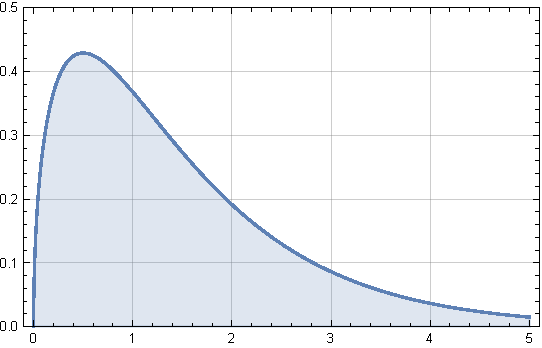
\includegraphics{Mathematica/output/SqrtExp.pdf}
    \end{Figure}
    因此,如果我们将\xrefpeq{7}的积分上限由$x'$改为$\infty$,并不会有太大的误差
    \begin{Equation}&[8]
        I=\Int[0][\infty]x^{1/2}\e^{-x}\dd{x}
    \end{Equation}
    而转化为无穷后,我们就可以将其向高斯积分的方向转化了,令$t=x^{1/2}$,则$\dd{x}=2t\dd{t}$
    \begin{Equation}&[9]
        I=2\Int[0][\infty]t^2\e^{-t^2}\dd{t}
    \end{Equation}
    而高斯积分的结论告诉我们
    \begin{Equation}&[10]
        I=2\frac{\sqrt{\pi}}{4}=\frac{\sqrt{\pi}}{2}
    \end{Equation}
    将\xrefpeq{10}代入\xrefpeq{6}
    \begin{Equation}&[11]
        n_0=\frac{1}{4\pi^{3/2}}\frac{(2\mne)^{3/2}}{\hbar^3}(\kB T)^{3/2}\exp(\frac{E_\text{F}-E_\text{c}}{\kB T})
    \end{Equation}
    我们可以将系数整理为一个统一的$3/2$次项
    \begin{Equation}&[12]
        n_0=\frac{1}{4}\qty(\frac{2\mne\kB T}{\pi\hbar^2})^{3/2}\exp(\frac{E_\text{F}-E_\text{c}}{\kB T})
    \end{Equation}
    我们在系数的括号内除以$4$,这相当于在括号外要乘$4^{3/2}=8$
    \begin{Equation}&[13]
        n_0=2\qty(\frac{\mne\kB T}{2\pi\hbar^2})^{3/2}\exp(\frac{E_\text{F}-E_\text{c}}{\kB T})
    \end{Equation}
    若记\xrefpeq{13}左端的常系数为$N_\text{c}$,我们就可以得到\xrefpeq{A}的结论形式,而依据\fancyref{fml:玻尔兹曼分布},此时\xrefpeq{13}右端的指数项$\exp(E_\text{F}-E_\text{c}/\kB T)$,其实也可以记为$f(E_\text{c})$。
\end{Proof}

\subsection{价带空穴浓度}
\begin{BoxFormula}[价带空穴浓度]
    价带空穴浓度满足
    \begin{Equation}&[A]
        p_0=N_\text{v}\exp(\frac{E_\text{v}-E_\text{F}}{\kB T})=N_\text{v}[1-f(E_\text{v})]
    \end{Equation}
    其中$N_\text{v}$称为价带的有效状态密度,满足
    \begin{Equation}&[B]
        N_\text{v}=2\qty(\frac{\mpe\kB T}{2\pi\hbar^2})^{3/2}
    \end{Equation}
\end{BoxFormula}

\begin{Proof}
    我们仍然从\xrefpeq[载流子浓度]{2}出发,但是这一次$f(E)$需要更换为$1-f(E)$,而$g_\text{c}(E)$需要换为$g_\text{v}(E)$
    \begin{Equation}&[1]
        \dd{n}=\frac{\dd{N}}{V}=\frac{[1-f(E)]g_\text{v}(E)}{V}
    \end{Equation}
    根据\fancyref{fml:价带顶的状态密度}和\fancyref{fml:玻尔兹曼分布}
    \begin{Equation}&[2]
        \dd{n}=\frac{1}{V}\qty[\frac{V}{2\pi^3}\frac{(2\mpe)^{3/2}}{\hbar^3}(E_\text{v}-E)^{1/2}]\qty[\exp(\frac{E-E_\text{F}}{\kB T})]
    \end{Equation}
    将$V$约掉,并对指数部分做一些调整
    \begin{Equation}&[3]
        \dd{n}=\frac{1}{2\pi^2}\frac{(2\mpe)^{3/2}}{\hbar^3}(E_\text{v}-E)^{1/2}\exp(\frac{E_\text{v}-E_\text{F}}{\kB T})\exp(\frac{E-E_\text{v}}{\kB T})
    \end{Equation}
    现在,让我们对$\dd{n}$进行积分
    \begin{Equation}&[4]
        \qquad\qquad
        p_0=\frac{1}{2\pi^2}\frac{(2\mpe)^{3/2}}{\hbar^3}\exp(\frac{E_\text{v}-E_\text{F}}{\kB T})\Int[E_\text{v}'][E_\text{v}]\exp(\frac{E-E_\text{v}}{\kB T})(E_\text{v}-E)^{1/2}\dd{E}
        \qquad\qquad
    \end{Equation}
    后续的步骤是完全相似的,积分后化简为
    \begin{Equation}&[5]
        p_0=2\qty(\frac{\mpe\kB T}{2\pi\hbar^2})^{3/2}\exp(\frac{E_\text{v}-E_\text{F}}{\kB T})
    \end{Equation}
    若记\xrefpeq{5}左端的常系数为$N_\text{v}$,我们就可以得到\xrefpeq{A}的结论形式,而依据\fancyref{fml:玻尔兹曼分布},此时\xrefpeq{5}右端的指数项$\exp(E_\text{v}-E_\text{F}/\kB T)$,其实亦可记为$1-f(E_\text{v})$。
\end{Proof}

\subsection{载流子的浓度乘积}
\begin{BoxFormula}[载流子的浓度乘积]
    载流子的浓度乘积满足
    \begin{Equation}
        n_0p_0=N_\text{c}N_\text{v}\exp(-\frac{E_\text{g}}{\kB T})
    \end{Equation}
    或者展开$N_\text{c},N_\text{v}$
    \begin{Equation}
        n_0p_0=4T^3\qty(\mne\mpe)^{3/2}\qty(\frac{\kB}{2\pi\hbar^2})^3\exp(-\frac{E_\text{g}}{\kB T})
    \end{Equation}
\end{BoxFormula}
\begin{Proof}
    这很容易证明,根据\fancyref{fml:导带电子浓度}和\fancyref{fml:价带空穴浓度}
    \begin{Equation}&[1]
        n_0p_0=N_\text{c}N_\text{v}\exp(\frac{E_\text{F}-E_\text{c}}{\kB T})\exp(\frac{E_\text{v}-E_\text{F}}{\kB T})
    \end{Equation}
    合并两个指数项
    \begin{Equation}&[2]
        n_0p_0=N_\text{c}N_\text{v}\exp(\frac{E_\text{v}-E_\text{c}}{\kB T})
    \end{Equation}
    我们知道禁带宽度$E_\text{g}=E_\text{c}-E_\text{v}$
    \begin{Equation}*
        n_0p_0=N_\text{c}N_\text{v}\exp(-\frac{E_\text{g}}{\kB T})\qedhere
    \end{Equation}
\end{Proof}

\fancyref{fml:载流子的浓度乘积}告诉我们一个重要的事实,\empx{电子和空穴的浓度乘积与费米能级无关}。该结论普遍适用于一切热平衡状态下的非简并半导体,且对本征半导体和杂质半导体都成立。实际上,掺杂改变的主要就是费米能级,故对于某种半导体材料,掺杂与否,掺杂的多少,并不会改变$n_0p_0$的结果,这会为我们之后讨论杂质半导体带来很多便利,比如
\begin{itemize}
    \item 如果掺杂使得电子浓度增加,那么空穴浓度必然会减少。
    \item 如果掺杂使得空穴浓度增加,那么空穴浓度必然会减少。
\end{itemize}
该结论还指出$n_0p_0$大致正比于$T^3$(在$T$较大时$\exp(-E_\text{g}/\kB T)$将趋向于$1$),这就表明,载流子的浓度乘积会随着温度增加而迅速增加,换言之,温度对于半导体的导电性的影响很大。
\section{本征半导体的载流子浓度}
\uwave{本征半导体}(Intrinsic Semiconductor)就是指一块没有杂质和缺陷的半导体,因此,本征半导体的载流子完全来自本征激发,由于本征激发中,电子从价带跃迁到导带,电子和空穴将会成对产生,因此,导带中的电子浓度应当等同于价带中的空穴浓度,这就是\uwave{电中性条件}。

\begin{BoxFormula}[本征半导体的电中性条件]
    本征半导体的电中性条件满足
    \begin{Equation}
        n_0=p_0
    \end{Equation}
\end{BoxFormula}

本征半导体的能带图,如\xref{fig:本征半导体的能带图}所示,其中,需要特别解释的是最右侧的图像,我们可能会困惑其中的$\dv*{n_0}{E}$和$\dv*{p_0}{E}$究竟是什么含义?介于$n_0$和$p_0$本身就是对能量$E$积分后的常数,又何谈对$E$的导数呢?实际上,在\xref{sec:载流子浓度}当我们通过积分求得$n_0$和$p_0$时,被积函数就是$f(E)g(E)/V$,它表征了载流子浓度的能量密度。原先的观点中$n_0,p_0$由能带底到能带顶的定积分,如果放宽一些,将$n_0,p_0$视为由能带顶到$E$的变上限积分$n_0(E),p_0(E)$,那这里的$\dv*{n_0}{E}$和$\dv*{p_0}{E}$就可以解释了,它们与$f(E)g(E)/V$是同一回事,都代表浓度的能量密度。这也是为何$f(E)g(E)/V$的曲线下面积就表示了电子浓度$n_0$和空穴浓度$p_0$的大小。
\begin{Figure}[本征半导体的能带图]
    \includegraphics[width=0.95\linewidth]{build/Chapter03D_03.fig.pdf}
\end{Figure}

这里也证实了先前的一个提法,我们注意到
\begin{itemize}
    \item 导带电子浓度的能量密度的最大值接近导带底,表明,\empx{导带电子主要位于导带底}。
    \item 价带电子浓度的能量密度的最大值接近价带顶,表明,\empx{价带空穴主要位于价带顶}。
\end{itemize}
这里关注到\xref{fig:本征半导体的能带图}中$f(E)$和$g(E)$的图像相较\xref{fig:状态密度函数}和\xref{fig:费米分布与玻尔兹曼分布},作为自变量的能量反而变为了纵轴,这其实是为了顺应简单能带图中,能量在纵向分布的习惯,也是半导体物理的通用作法。


至此,有一个疑惑,这一节我们到底要干嘛?本节题名“本征半导体的载流子浓度”,但问题是,载流子的浓度我们在\xref{sec:载流子浓度}中,已经由\fancyref{fml:导带电子浓度}和\fancyref{fml:价带空穴浓度}求出了,本节还有什么可做的?关键点在于,现有的$n_0$和$p_0$的公式中包含费米能级$E_\text{F}$,而根据固体物理的知识,\empx{费米能级是随温度变化的函数},而这个函数是我们目前未知的。因此,本节就是要求出本征半导体的费米能级的函数,进而求出$n_0$和$p_0$的具体表达。

\begin{BoxFormula}[本征半导体的费米能级]*
    本征半导体的费米能级满足
    \begin{Equation}
        E_\text{F}=\frac{E_\text{c}-E_\text{v}}{2}+\frac{\kB T}{2}\ln\frac{N_\text{v}}{N_\text{c}}
    \end{Equation}
    或
    \begin{Equation}
        E_\text{F}=E_\text{i}=\frac{E_\text{c}+E_\text{v}}{2}+\frac{3\kB T}{4}\ln\frac{\mpe}{\mne}
    \end{Equation}
    这里$E_\text{i}$是专属本征半导体的费米能级的记号,下标i表示本征(Intrinsic)。
\end{BoxFormula}
\begin{Proof}
    求解费米能级的关键,在于运用电中性条件,根据\fancyref{fml:本征半导体的电中性条件}
    \begin{Equation}&[1]
        n_0=p_0
    \end{Equation}
    根据\fancyref{fml:导带电子浓度}和\fancyref{fml:价带空穴浓度}
    \begin{Equation}&[2]
        N_\text{c}\exp(\frac{E_\text{F}-E_\text{c}}{\kB T})=N_\text{v}\exp(\frac{E_\text{v}-E_\text{F}}{\kB T})
    \end{Equation}
    在\xrefpeq{2}两端取对数
    \begin{Equation}&[3]
        \ln N_\text{c}+\qty(\frac{E_\text{F}-E_\text{c}}{\kB T})=\ln N_\text{V}+\qty(\frac{E_\text{v}}{\kB T})
    \end{Equation}
    移项整理
    \begin{Equation}&[4]
        \frac{2E_\text{F}-E_\text{c}-E_\text{v}}{\kB T}=\ln\frac{N_\text{v}}{N_\text{c}}
    \end{Equation}
    再整理
    \begin{Equation}&[5]
        \frac{2E_\text{F}}{\kB T}=\frac{E_\text{c}-E_\text{v}}{\kB T}+\ln\frac{N_\text{v}}{N_\text{c}}
    \end{Equation}
    由此即解得$E_\text{F}$
    \begin{Equation}&[6]
        E_\text{F}=\frac{E_\text{c}-E_\text{v}}{2}+\frac{\kB T}{2}\ln\frac{N_\text{v}}{N_\text{c}}
    \end{Equation}
    而我们知道$N_\text{v}\sim(\mpe)^{3/2}$和$N_\text{c}\sim(\mne)^{3/2}$
    \begin{Equation}&[7]
        E_\text{F}=\frac{E_\text{c}-E_\text{v}}{2}+\frac{3\kB T}{4}\ln\frac{\mpe}{\mne}
    \end{Equation}
    这里,我们愿意引入$E_\text{i}$作为本征半导体中费米能级$E_\text{F}$的特别记号。
\end{Proof}

\xref{fml:本征半导体的费米能级}指出,本征半导体的费米能级$E_\text{i}$由两部分组成,首先是$E_\text{c}+E_\text{v}/2$的常数部分,它表明费米能级在绝对零度时位于禁带中线上,其次是$(3\kB T/4)\ln(\mpe/\mne)$的线性项,它表明费米能级将随温度增大线性变化。不过事实上,对于大部分半导体材料,在室温范围内,线性项的影响其实都不大。例如,根据\xref{tab:半导体的状态密度有效质量}的数据,硅和锗的$\mpe/\mne$分别为$0.55$和$0.52$,砷化镓的$\mpe/\mne$则为$8.25$,故三者的$\ln(\mpe/\mne)$均大致在$\pm 2$的范围内,而$\kB T$在室温$T=300\si{K}$时为$\kB T=0.026\si{eV}$,因此整个线性项在室温下的影响小于$0.05\si{eV}$,根据\xref{tab:部分半导体材料的参数}的数据,其相较于硅、锗、砷化镓$1.14\si{eV}, 0.67\si{eV}, 1.52\si{eV}$在$1\si{eV}$量级的禁带宽度,完全可以忽略,因此我们可以近似认为,\empx{本征半导体的费米能级基本在禁带中线附近}。不过,也有例外,例如锑化铟的$\mpe/\mne$约为$36.7$,取对数后仍然有$3.60$,线性项的影响达到了近$0.07\si{eV}$,但是,锑化铟的禁带非常窄,仅有$0.17\si{eV}$,这时,线性项的影响就很显著了,费米能级已远在禁带中线上了。

现在,让我们来计算本征半导体的载流子浓度。

\begin{BoxFormula}[本征半导体的载流子浓度]
    本征半导体中,电子浓度$n_0$和空穴浓度$p_0$相等,统一记为$n_\text{i}$
    \begin{Equation}
        n_\text{i}=n_0=p_0
    \end{Equation}
    且$n_\text{i}$满足
    \begin{Equation}
        n_\text{i}=(N_\text{c}N_\text{v})^{1/2}\exp(-\frac{E_\text{g}}{2\kB T})
    \end{Equation}
\end{BoxFormula}

\begin{Proof}
    根据\fancyref{fml:导带电子浓度},并代入\fancyref{fml:本征半导体的费米能级}
    \begin{Equation}&[1]
        \qquad
        n_0=N_\text{c}\exp(\frac{E_\text{F}-E_\text{c}}{\kB T})=N_\text{c}\exp(\frac{E_\text{c}/2+E_\text{v}/2+(\kB T/2)\ln N_\text{v}/N_\text{c}-E_\text{c}}{\kB T})
        \qquad
    \end{Equation}
    化简整理得
    \begin{Equation}&[2]
        n_0=N_\text{c}\qty(-\frac{E_\text{c}-E_\text{v}}{2\kB T}+\frac{\ln N_\text{v}/N_\text{c}}{2})=N_\text{c}\sqrt{N_\text{v}/N_\text{c}}\exp(-\frac{E_\text{g}}{2\kB T})=(N_\text{c}N_\text{v})^{1/2}\exp(-\frac{E_\text{g}}{2\kB T})
    \end{Equation}
    根据\fancyref{fml:价带空穴浓度},并代入\fancyref{fml:本征半导体的费米能级}
    \begin{Equation}&[3]
        \qquad
        p_0=N_\text{v}\exp(\frac{E_\text{v}-E_\text{F}}{\kB T})=N_\text{c}\exp(\frac{E_\text{v}-E_\text{c}/2-E_\text{v}/2-(\kB T/2)\ln N_\text{v}/N_\text{c}}{\kB T})
        \qquad
    \end{Equation}
    化简整理得
    \begin{Equation}&[4]
        p_0=N_\text{v}\qty(-\frac{E_\text{c}-E_\text{v}}{2\kB T}-\frac{\ln N_\text{v}/N_\text{c}}{2})=N_\text{v}\sqrt{N_\text{c}/N_\text{v}}\exp(-\frac{E_\text{g}}{2\kB T})=(N_\text{v}N_\text{c})^{1/2}\exp(-\frac{E_\text{g}}{2\kB T})
    \end{Equation}
    比较\xrefpeq{3}和\xrefpeq{4}即得
    \begin{Equation}*
        n_0=p_0\qedhere
    \end{Equation}
\end{Proof}
由此可见,本征半导体的载流子浓度对温度非常敏感,其随温度增加而迅速增加。而在同一温度下,半导体材料的禁带宽度$E_\text{g}$越大,本征载流子的浓度$n_i$就相应越小,这从直观上想也是很合理的,因为禁带宽度越大,电子从价带跃迁到导带也越困难,载流子自然也就少了。

在\xref{fml:本征半导体的载流子浓度}中代入$N_\text{c}N_\text{v}$,并引入\fancyref{fml:禁带宽度和温度的关系}
\begin{Equation}
    n_i=2\frac{(2\pi \kB T)^{3/2}(\mpe\mne)^{3/4}}{\hbar^3}\exp[-\frac{E_\text{g}(0)}{2\kB T}]\exp[\frac{\alpha T}{2\kB (T+\beta)}]
\end{Equation}
该式可以在实验上用于测定禁带宽度。
\section{杂质半导体的载流子浓度}
\uwave{杂质半导体}(Extrinsic Semiconductor)是指人为引入杂质后的半导体,杂质的电离将会影响原有的载流子分布。但是,杂质并不是什么奇妙的魔法,如\xref{fig:杂质半导体的能带图}所示,杂质半导体的状态密度$g(E)$与本征半导体完全一致,杂质半导体的概率密度$f(E)$仍然遵从费米分布,那么到底什么被改变了?使杂质型半导体,表现出与本征半导体不同的载流子浓度?答案是费米能级
\begin{itemize}
    \item N型半导体的费米能级较靠近导带底,使导带电子浓度增加,使价带空穴减小。
    \item P型半导体的费米能级较靠近价带顶,使价带空穴浓度增加,使导带电子减小。
\end{itemize}
\begin{Figure}[杂质半导体的能带图]
    \begin{FigureSub}[N型半导体]
        \includegraphics[width=0.95\linewidth]{build/Chapter03D_04.fig.pdf}
    \end{FigureSub}\vspace{0.5cm}
    \begin{FigureSub}[P型半导体]
        \includegraphics[width=0.95\linewidth]{build/Chapter03D_05.fig.pdf}
    \end{FigureSub}
\end{Figure}
那么,为什么掺杂会导致费米能级的行为发生变化呢?根据\xref{sec:本征半导体的载流子浓度},载流子的电中性条件决定费米能级,载流子的浓度又反过来由费米能级确定。所以,可以肯定的是,\empx{掺杂会以某种方式干预了电中性条件},尽管我们无法直接确定杂质会如何影响浓度分布,但是,掺入了多少杂质,掺入的杂质中有多少会发生电离,这是可以理论计算的,由此就能得到新的电中性条件。

\subsection{杂质能级上的电子和空穴}
那么首先要解决的问题是,掺入的杂质中有多少比例发生电离?其实,我们不妨换一个问法
\begin{itemize}
    \item 电子占据施主能级的概率$f_\text{D}(E_\text{D})$为多少?
    \item 空穴占据受主能级的概率$f_\text{A}(E_\text{A})$为多少?
\end{itemize}
当电子或空穴占据施主能级或受主能级时,这就是杂质没有电离的状态,我们关心的是杂质发生电离,向导带或价带输送电子或空穴的概率,这分别由$1-f_\text{D}(E_\text{D})$和$1-f_\text{A}(E_\text{A})$给出。

但现在的问题是,我们知道,费米分布$f(E)$事实上描述了电子占据某个能级的概率密度,那么,电子占据施主能级的概率$f_\text{D}(E_\text{D})$,空穴占据受主能级的概率$f_\text{A}(E_\text{A})$,是否也是服从费米分布的呢?遗憾的是,答案是否定的。因为杂质能级与能带中的能级是有区别,正如我们在\xref{subsec:施主杂质和受主杂质}所说,杂质能级是一系列具有相同能量的孤立能级,但是,其不同于能带中的能级可以由两个自旋相反的电子占有,杂质能级上只能进入一个任意自旋的电子,这是因为杂质原子也只能额外吸引一个电子,所以,\empx{杂质能级不服从费米分布}。有理论可以证明
\begin{BoxFormula}[施主能级的概率]
    电子占据施主能级的概率是
    \begin{Equation}
        f_\text{D}(E)=\frac{1}{1+g_\text{D}^{-1}\exp[(E_\text{D}-E_\text{F})/\kB T]}
    \end{Equation}
    其中,$g_\text{D}$是\uwave{施主能级的基态简并度}。
\end{BoxFormula}
\begin{BoxFormula}[受主能级的概率]
    空穴占据受主能级的概率是
    \begin{Equation}
        f_\text{A}(E)=\frac{1}{1+g_\text{A}^{-1}\exp[(E_\text{F}-E_\text{A})/\kB T]}
    \end{Equation}
    其中,$g_\text{A}$是\uwave{受主能级的基态简并度}。
\end{BoxFormula}
通常而言,对于硅、锗、砷化镓等材料,通常会取基态简并度(简并因子)为
\begin{Equation}
    g_\text{D}=2\qquad
    g_\text{A}=4
\end{Equation}
如果我们分别记施主浓度和受主浓度为$N_\text{D}$和$N_\text{A}$,那么就可以写出相关的浓度了,这里需要说明的是,所谓“电离施主浓度”和“电离受主浓度”,其实就是指由杂质发生电离,进入导带和价带的电子和空穴的浓度,它们等于相应杂质离子的浓度,故$n_\text{D}^{+}$和$p_\text{A}^{-}$就是我们所关心的。
\begin{BoxFormula}[施主浓度]
    施主能级上的电子浓度$n_\text{D}$和电离施主浓度$n_\text{D}^{+}$分别为
    \begin{Equation}
        n_\text{D}=N_\text{D}f_\text{D}(E_\text{D})\qquad 
        n_\text{D}^{+}=N_\text{D}[1-f_\text{D}(E_\text{D})]
    \end{Equation}
    其中$N_\text{D}$为掺入的施主杂质的浓度。
\end{BoxFormula}\nopagebreak
\begin{BoxFormula}[受主浓度]
    受主能级上的空穴浓度$p_\text{A}$和电离受主浓度$p_\text{A}^{-}$分别为
    \begin{Equation}
        p_\text{A}=N_\text{A}f_\text{A}(E_\text{A})\qquad 
        p_\text{A}^{-}=N_\text{A}[1-f_\text{A}(E_\text{A})]
    \end{Equation}
    其中$N_\text{A}$为掺入的受主杂质的浓度。
\end{BoxFormula}

\subsection{杂质半导体的电中性条件}
简洁起见,自本小节开始,我们都姑且以仅包含施主能级的N型半导体为例讨论。

杂质半导体中的杂质对电中性条件有何种影响?对于N型半导体,负电荷显然是由价带电子浓度$n_0$构成,这里面同时包含了本征激发和杂质电离的电子。正电荷则包含两部分,一部分来自导带空穴浓度$p_0$,一部分来自电离施主浓度$n_\text{D}^{+}$(考虑到电离后的施主离子带正电荷)。
\begin{BoxFormula}[杂质半导体的电中性条件]
    N型杂质半导体的电中性条件满足
    \begin{Equation}
        n_0=n_\text{D}^{+}+p_0
    \end{Equation}
\end{BoxFormula}
代入\fancyref{fml:导带电子浓度}、\fancyref{fml:价带空穴浓度}、\fancyref{fml:施主浓度}
\begin{Equation}
    \qquad\qquad
    N_\text{c}\exp(\frac{E_\text{F}-E_\text{c}}{\kB T})=
    N_\text{v}\exp(\frac{E_\text{v}-E_\text{F}}{\kB T})+
    \frac{N_\text{D}}{1+g_\text{D}\exp(E_\text{F}-E_\text{D}/\kB T)}
    \qquad\qquad
\end{Equation}
或许有些不自量力的人\footnote{没错是我……曾试图用Mathematica求解这个方程,但或许是由于技术不够娴熟,得到的解不知为何无法绘制出任何曲线,成功浪费了几个小时,一无所获,很郁闷。虽然如此,但确实很好奇这里费米能级$E_\text{F}$的精确解绘制成函数曲线,究竟会是何种样貌?}试图求解上面这个方程以得到$E_\text{F}$的表达式,事实上,经过恰当的变量代换,该方程大概可以转化为一个四次方程,而总所周知,四次方程的解是令人发指般的复杂,其实不利于我们把握简洁的物理图景。因而,我们需要做一些近似,我们会将$E_\text{F}(T)$的函数关系划分为若干个温度区间,在每个温度区间内适用相应的近似条件,从而简化电中性条件的表达式,由此得到若干适用不同温度范围的$E_\text{F}(T)$的表达式。这就是接下来我们要做的。

\subsection{低温弱电离区}
当温度很低时,大部分施主杂质能级仍然为电子所占据,只有很少量的施主杂质发生电离,这些极少量的电子进入导带,称为弱电离。而这种情况下,本征激发的电子就更加可以忽略了。
\begin{BoxDefinition}[低温弱电离区]
    \uwave{低温弱电离区}是指,施主杂质少量电离,本征激发可以忽略
    \begin{Equation}
        n_\text{D}^{+}\ll N_\text{D}\qquad
        p_0=0
    \end{Equation}
\end{BoxDefinition}

\begin{BoxFormula}[低温弱电离区的电中性条件]
    低温弱电离区适用的电中性条件为
    \begin{Equation}
        n_0=n_\text{D}^{+}
    \end{Equation}
    更具体的
    \begin{Equation}
        N_\text{c}\exp(\frac{E_\text{F}-E_\text{c}}{\kB T})=\frac{1}{g_\text{D}}N_\text{D}\exp(\frac{E_\text{D}-E_\text{F}}{\kB T})
    \end{Equation}
\end{BoxFormula}
\begin{Proof}
    根据\fancyref{fml:杂质半导体的电中性条件}
    \begin{Equation}&[1]
        n_0=n_\text{D}^{+}+p_0
    \end{Equation}
    根据\fancyref{def:低温弱电离区}中的$p_0=0$
    \begin{Equation}&[2]
        n_0=n_\text{D}^{+}
    \end{Equation}
    代入\fancyref{fml:导带电子浓度}和\fancyref{fml:施主浓度}
    \begin{Equation}&[3]
        N_\text{c}\exp(\frac{E_\text{F}-E_\text{c}}{\kB T})=\frac{N_\text{D}}{1+g_\text{D}\exp(E_\text{F}-E_\text{D}/\kB T)}
    \end{Equation}
    根据\fancyref{def:低温弱电离区}中的$n_0\ll N_\text{D}$,推定\xrefpeq{3}右端指数项必远大于$1$,故
    \begin{Equation}&[4]
        N_\text{c}\exp(\frac{E_\text{F}-E_\text{c}}{\kB T})=\frac{N_\text{D}}{g_\text{D}\exp(E_\text{F}-E_\text{D}/\kB T)}
    \end{Equation}
    因此
    \begin{Equation}*
        N_\text{c}\exp(\frac{E_\text{F}-E_\text{c}}{\kB T})=\frac{1}{g_\text{D}}N_\text{D}\exp(\frac{E_\text{D}-E_\text{F}}{\kB T})\qedhere
    \end{Equation}
\end{Proof}

而有了电中性条件后,计算费米能级就不是太困难的事情了。
\begin{BoxFormula}[低温弱电离区的费米能级]
    低温弱电离区的费米能级满足
    \begin{Equation}
        E_\text{F}=\frac{E_\text{c}+E_\text{D}}{2}+\qty(\frac{\kB T}{2})\ln\qty(\frac{N_\text{D}}{g_\text{D}N_\text{c}})
    \end{Equation}
\end{BoxFormula}
\begin{Proof}
    根据\fancyref{fml:低温弱电离区的电中性条件}
    \begin{Equation}&[1]
        N_\text{c}\exp(\frac{E_\text{F}-E_\text{c}}{\kB T})=\frac{1}{g_\text{D}}N_\text{D}\exp(\frac{E_\text{D}-E_\text{F}}{\kB T})
    \end{Equation}
    两端同时取对数
    \begin{Equation}&[2]
        \ln N_\text{c}+\frac{E_\text{F}-E_\text{c}}{\kB T}=\ln\frac{N_\text{D}}{g_\text{D}}+\frac{E_\text{D}-E_\text{F}}{\kB T}
    \end{Equation}
    移项整理
    \begin{Equation}&[3]
        \frac{2E_\text{F}-E_\text{c}-E_\text{D}}{\kB T}=\ln\frac{N_\text{D}}{g_\text{D}N_\text{c}}
    \end{Equation}
    再整理
    \begin{Equation}&[4]
        \frac{2E_\text{F}}{\kB T}=\frac{E_\text{c}+E_\text{D}}{\kB T}+\ln\frac{N_\text{D}}{g_\text{D}N_\text{c}}
    \end{Equation}
    即得
    \begin{Equation}*
        E_\text{F}=\frac{E_\text{c}+E_\text{D}}{2}+\qty(\frac{\kB T}{2})\ln\frac{N_\text{D}}{g_\text{D}N_\text{c}}\qedhere
    \end{Equation}
\end{Proof}

低温弱电离区的费米能级与温度的关系比较复杂(因为$N_\text{c}$同样与温度有关),分析如下。
\begin{BoxProperty}[低温弱电离区的费米能级的性质]
    低温弱电离区的费米能级$E_\text{F}(T)$随温度增加,先增大,后减小。

    当$T\to 0\si{K}$时,费米能级趋近导带底和杂质能级的中线
    \begin{Equation}
        \Lim[T\to 0]E_\text{F}(T)=\frac{E\text{c}+E_\text{D}}{2}
    \end{Equation}
    在$N_\text{c}$满足下左式时(此时$T$满足下右式),费米能级取最大值
    \begin{Equation}
        N_\text{c}=\qty(\frac{N_\text{D}}{g_\text{D}})\e^{-3/2}\qquad
        T=\frac{2\pi\hbar^2}{\mne\kB\e}\qty(\frac{N_\text{D}}{2g_\text{D}})^{2/3}
    \end{Equation}
    在$N_\text{c}$满足下左式时(此时$T$满足下右式),费米能级回落到中线
    \begin{Equation}
        N_\text{c}=\qty(\frac{N_\text{D}}{g_\text{D}})\qquad
        T=\frac{2\pi\hbar^2}{\mne\kB}\qty(\frac{N_\text{D}}{2g_\text{D}})^{2/3}
    \end{Equation}
\end{BoxProperty}

\begin{Proof}
    \paragraph{讨论绝对零度时的结论}
    根据\fancyref{fml:低温弱电离区的费米能级}
    \begin{Equation}&[1]
        E_\text{F}=\frac{E_\text{c}+E_\text{D}}{2}+\qty(\frac{\kB T}{2})\ln\qty(\frac{N_\text{D}}{g_\text{D}N_\text{c}})
    \end{Equation}
    根据\fancyref{fml:导带电子浓度}
    \begin{Equation}&[2]
        N_\text{c}=2\qty(\frac{\mne\kB T}{2\pi\hbar^2})^{3/2}
    \end{Equation}
    这就是说
    \begin{Equation}&[3]
        N_\text{c}\propto T^{3/2}
    \end{Equation}
    将\xrefpeq{3}中$N_\text{c}$代回\xrefpeq{1},注意到$T\to 0$时$T\ln(T^{-3/2})\to 0$,故
    \begin{Equation}&[4]
        \Lim[T\to 0]E_\text{F}(T)=\frac{E_\text{c}+E_\text{D}}{2}
    \end{Equation}
    \paragraph{讨论费米能级取何时最大值}
    接下来,我们通过对$E_\text{F}$求导来分析$E_\text{F}$的性质
    \begin{Equation}&[5]
        \dv{E_\text{F}}{T}=\frac{\kB}{2}\ln\qty(\frac{N_\text{D}}{g_\text{D}N_\text{c}})+\frac{\kB T}{2}\dv{T}\ln\qty(\frac{N_\text{D}}{g_\text{D}N_\text{c}})
    \end{Equation}
    运用复合函数的导数法则
    \begin{Equation}&[6]
        \dv{E_\text{F}}{T}=\frac{\kB}{2}\ln\qty(\frac{N_\text{D}}{g_\text{D}N_\text{c}})+\frac{\kB T}{2}\qty[\frac{g_\text{D}N_\text{c}}{N_\text{D}}\cdot\frac{N_\text{D}}{g_\text{D}}\cdot\dv{T}\qty(\frac{1}{N_\text{c}})]
    \end{Equation}
    化简整理得
    \begin{Equation}&[7]
        \dv{E_\text{F}}{T}=\frac{\kB}{2}\ln\qty(\frac{N_\text{D}}{g_\text{D}N_\text{c}})+\frac{\kB T}{2}\qty[N_\text{c}\dv{T}\qty(\frac{1}{N_\text{c}})]
    \end{Equation}
    而根据$1/N_\text{c}\propto T^{-3/2}$
    \begin{Equation}&[8]
        T\dv{T}\qty(\frac{1}{N_\text{c}})=-\frac{3}{2}\qty(\frac{1}{N_\text{c}})
    \end{Equation}
    将\xrefpeq{8}代回\xrefpeq{7}
    \begin{Equation}&[9]
        \dv{E_\text{F}}{T}=\frac{\kB}{2}\ln\qty(\frac{N_\text{D}}{g_\text{D}N_\text{c}})-\frac{\kB}{2}\cdot\frac{3}{2}
    \end{Equation}
    即
    \begin{Equation}&[10]
        \dv{E_\text{F}}{T}=\frac{\kB}{2}\qty[\ln\qty(\frac{N_\text{D}}{g_\text{D}N_\text{c}})-\frac{3}{2}]
    \end{Equation}
    我们注意到,如果$N_\text{c}$满足下式,一阶导数$\dv*{E_\text{F}}{T}$为零
    \begin{Equation}&[11]
        \ln(\frac{N_\text{D}}{g_\text{D}N_\text{c}})=\frac{3}{2}\qquad N_\text{c}=\qty(\frac{N_\text{D}}{g_\text{D}})\e^{-3/2}
    \end{Equation}
    依据\xrefpeq{2}不难求出此时$T$应当满足的值。

    \paragraph{讨论费米能级何时回落至中线}
    最后的问题是容易,让我们回归\xrefpeq{1},注意到$N_\text{c}$满足下式时有$E_\text{F}=(E_\text{c}+E_\text{D})/2$
    \begin{Equation}
        \ln(\frac{N_\text{D}}{g_\text{D}N_\text{c}})=0\qquad N_\text{c}=\qty(\frac{N_\text{D}}{g_\text{D}})
    \end{Equation}
    依据\xrefpeq{2}不难求出此时$T$应当满足的值。
\end{Proof}

\xref{fig:杂质半导体的费米能级}形象的展现了低温电离区费米能级如何随温度变化
\begin{Figure}[杂质半导体的特性]
    \begin{FigureSub}[杂质半导体的费米能级]
        \includegraphics[scale=0.85]{build/Chapter03D_01.fig.pdf}
    \end{FigureSub}
    \vspace{0.35cm}
    \begin{FigureSub}[杂质半导体的载流子浓度]
        \includegraphics[scale=0.85]{build/Chapter03D_02.fig.pdf}
    \end{FigureSub}
\end{Figure}
\xref{fig:杂质半导体的费米能级}中分别用$T_1,T_2$标识\xref{ppt:低温弱电离区的费米能级的性质}中,费米能级取最大值和回落到中线时的温度。

\xref{fig:杂质半导体的费米能级}在绘图时,取有效质量比$\mpe/\mne\approx 0.5$,取禁带宽度$E_\text{g}=1.0\si{eV}$,这是接近硅和锗的参数值,由此计算出的室温$300\si{K}$下的$N_\text{c}$在$1\times 10^{19}\si{cm^{-3}}$的数量级,而通常来说,作为非简并半导体,掺杂的浓度$N_\text{D}$应当满足$N_\text{D}\ll N_\text{c}$\;。但是,由于这里我们希望绘制一张能全面反映各个温度区段的费米能级变化趋势的示意图像,如果真的取$N_\text{D}\ll N_\text{c}$,低温弱电离区的特性在整体尺度上将完全不可见,例如,如果我们取$N_\text{D}=1\times 10^{16}\si{cm^{-3}}$,则$T_1,T_2$的值甚至不足$1\si{K}$,并且低温弱电离区$E_\text{F}$的最大值与$(E_\text{c}+E_\text{D})/2$的中线的间距几乎为零,使低温弱电离区的特性都无法被体现。为了凸显低温弱电离区的特性,我们被迫将掺杂浓度提高到了不合理的$N_\text{c}=1\times 10^{20}\si{cm^{-3}}$,很明显,这导致了诸多荒谬。首先,这个掺杂浓度不再符合非简并半导体的近似假设,需要适用简并半导体的理论。其次,低温弱电离区的特性范围至少可以延伸到$300\si{K}$的室温,这是不符合实际的,更明显的是,本征特性需要在高达$4000\si{K}$左右的高温才能显现,这个温度下任何半导体都已经融化了。但总之,作为一张示意图,它是成功的。

现在,有了低温弱电离区的费米能级,我们就可以计算低温弱电离区的载流子浓度了。
\begin{BoxFormula}[低温弱电离区的载流子浓度]*
    低温弱电离区中,导带电子浓度满足
    \begin{Equation}
        n_0=\qty(\frac{N_\text{D}N_\text{c}}{g_\text{D}})^{1/2}\exp(-\frac{\delt{E_\text{D}}}{2\kB T})
    \end{Equation}
    低温弱电离区中,价带空穴浓度满足
    \begin{Equation}
        p_0=0
    \end{Equation}
\end{BoxFormula}
\begin{Proof}
    根据\fancyref{fml:导带电子浓度}
    \begin{Equation}
        n_0=N_\text{c}\exp(\frac{E_\text{F}-E_\text{c}}{\kB T})
    \end{Equation}
    代入\fancyref{fml:低温弱电离区的费米能级}
    \begin{Equation}
        n_0=N_\text{c}\exp[\frac{(E_\text{c}+E_\text{D})/2+(\kB T/2)\ln(N_\text{D}/g_\text{D}N_\text{c})-E_\text{c}}{\kB T}]
    \end{Equation}
    化简得到
    \begin{Equation}
        n_0=N_\text{c}\exp[\frac{E_\text{D}-E_\text{c}}{2\kB T}+\frac{1}{2}\ln(\frac{N_\text{D}}{g_\text{D}N_\text{c}})]
    \end{Equation}
    即
    \begin{Equation}
        n_0=N_\text{c}\exp(\frac{E_\text{D}-E_\text{c}}{2\kB T})\qty(\frac{N_\text{D}}{g_\text{D}N_\text{c}})^{1/2}
    \end{Equation}
    整理,应用$\delt{E_\text{D}}=E_\text{c}-E_\text{D}$
    \begin{Equation}
        n_0=\exp(-\frac{\delt{E_\text{D}}}{2\kB T})\qty(\frac{N_\text{D}N_\text{c}}{g_\text{D}})^{1/2}\qedhere
    \end{Equation}
    这就求得了$n_0$,而$p_0=0$是由\fancyref{def:低温弱电离区}直接得到的。
\end{Proof}
由于$N_\text{c}\propto T^{3/2}$,因此$n_0\propto T^{3/4}\exp(-1/T)$,当$T$较大时$n_0\propto T^{3/4}$,如\xref{fig:杂质半导体的载流子浓度}所示。

\subsection{高温强电离区}
当温度较高时,大部分施主杂质都发生电离,称为强电离,此时本征激发仍然可以忽略。

\begin{BoxDefinition}[高温强电离区]
    高温强电离区是指,施主杂质全部电离,本征激发可以忽略
    \begin{Equation}
        n_\text{D}^{+}=N_\text{D}\qquad
        p_0=0
    \end{Equation}
\end{BoxDefinition}

\begin{BoxFormula}[高温强电离区的电中性条件]
    高温强电离区的电中性条件为
    \begin{Equation}
        n_0=n_\text{D}^{+}
    \end{Equation}
    更具体的
    \begin{Equation}
        N_\text{c}\exp(\frac{E_\text{F}-E_\text{c}}{\kB T})=N_\text{D}
    \end{Equation}
\end{BoxFormula}
\begin{Proof}
    根据\fancyref{fml:杂质半导体的电中性条件}
    \begin{Equation}
        n_0=n_\text{D}^{+}+p_0
    \end{Equation}
    根据\fancyref{def:高温强电离区}中的$p_0=0$
    \begin{Equation}
        n_0=n_\text{D}^{+}
    \end{Equation}
    根据\fancyref{fml:导带电子浓度}和\fancyref{def:高温强电离区}的$n_\text{D}^{+}=N_\text{D}$
    \begin{Equation}*
        N_\text{c}\exp(\frac{E_\text{F}-E_\text{c}}{\kB T})=N_\text{D}\qedhere
    \end{Equation}
\end{Proof}
而有了电中性条件后,计算费米能级就不是太困难的事情了。
\begin{BoxFormula}[高温强电离区的费米能级]
    高温强电离区的费米能级满足
    \begin{Equation}
        E_\text{F}=E_\text{c}+\kB T\ln(\frac{N_\text{D}}{N_\text{c}})
    \end{Equation}
\end{BoxFormula}
\begin{Proof}
    根据\fancyref{fml:高温强电离区的电中性条件}
    \begin{Equation}&[1]
        N_\text{c}\exp(\frac{E_\text{F}-E_\text{c}}{\kB T})=N_\text{D}
    \end{Equation}
    两端同时取对数
    \begin{Equation}&[2]
        \ln N_\text{c}+\frac{E_\text{F}-E_\text{c}}{\kB T}=\ln N_\text{D}
    \end{Equation}
    移项整理得
    \begin{Equation}*
        E_\text{F}=E_\text{c}+\kB T\ln(\frac{N_\text{D}}{N_\text{c}})\qedhere
    \end{Equation}
\end{Proof}
如\xref{fig:杂质半导体的费米能级}所示,高温强电离区和低温弱电离区的曲线是相似的,这是因为,如果我们仔细对比\xref{fml:低温弱电离区的费米能级}和\xref{fml:高温强电离区的费米能级},我们会发现,强电离区和弱电离区中,费米能级的函数形式是一致的,只不过参数有些不同。不过,高温强电离区中我们并不关心随温度先增大后减小的那部分特性,因为那里的温度低于高温强电离区的近似适用范围。另外,注意到,高温强电离区的曲线和低温弱电离区的曲线是无法相接的,这是因为两者实质都是不考虑本征激发的电中性条件$n_0=n_\text{D}^{+}$的极限情况,低温弱电离区假定$n_\text{D}^{+}\ll N_\text{D}$,高温强电离区则假定$n_\text{D}^{+}=N_\text{D}$。

\begin{BoxFormula}[高温强电离区的载流子浓度]
    高温强电离区中,导带电子浓度满足
    \begin{Equation}
        n_0=N_\text{D}
    \end{Equation}
    高温强电离区中,价带空穴浓度满足
    \begin{Equation}
        p_0=0
    \end{Equation}
\end{BoxFormula}
\begin{Proof}
    由\fancyref{def:高温强电离区}和\fancyref{fml:高温强电离区的电中性条件}立即得到。
\end{Proof}
如\xref{fig:杂质半导体的特性}所示,高温强电离区的电子浓度是常数,始终等于杂质浓度$N_\text{D}$。

现在的问题是,尽管我们不能精确求解弱电离区和强电离区间的中间状态,但是我们尚可以通过一些分析,确定杂质何时可以视为完全电离,换言之,确定何时可以适用强电离区的模型。

\begin{BoxFormula}[未电离的施主浓度]*
    未电离的施主浓度$n_\text{D}$可以表示为
    \begin{Equation}
        n_\text{D}=D_{-}N_\text{D}
    \end{Equation}
    其中$D_{-}$为
    \begin{Equation}
        D_{-}=\qty(\frac{g_\text{D}N_\text{D}}{N_\text{c}})\exp(\frac{\delt{E_\text{D}}}{\kB T})
    \end{Equation}
\end{BoxFormula}

\begin{Proof}
    根据\fancyref{fml:施主浓度}和\fancyref{fml:施主能级的概率}
    \begin{Equation}
        n_\text{D}=N_\text{D}f_\text{D}(E_\text{D})=\frac{N_\text{D}}{1+g_\text{D}^{-1}\exp[(E_\text{D}-E_\text{F})/\kB T]}
    \end{Equation}
    当$E_\text{D}-E_\text{F}\gg \kB T$时\footnote{为什么高温强电离区能满足这个近似条件呢?}
    \begin{Equation}
        n_\text{D}=g_\text{D}N_\text{D}\exp(\frac{E_\text{F}-E_\text{D}}{\kB T})
    \end{Equation}
    将\fancyref{fml:高温强电离区的费米能级}代入
    \begin{Equation}
        n_\text{D}=g_\text{D}N_\text{D}\exp[\frac{E_\text{c}+\kB T\ln(N_\text{D}/N_\text{c})-E_\text{D}}{\kB T}]
    \end{Equation}
    即
    \begin{Equation}
        n_\text{D}=g_\text{D}N_\text{D}\exp(\frac{E_\text{c}-E_\text{D}}{\kB T})\frac{N_\text{D}}{N_\text{c}}
    \end{Equation}
    整理得
    \begin{Equation}
        n_\text{D}=\qty(\frac{g_\text{D}N_\text{D}}{N_\text{c}})\exp(\frac{\delt{E_\text{D}}}{\kB T})N_\text{D}
    \end{Equation}
    如果我们愿意记
    \begin{Equation}
        D_{-}=\qty(\frac{g_\text{D}N_\text{D}}{N_\text{c}})\exp(\frac{\delt{E_\text{D}}}{\kB T})
    \end{Equation}
    那么
    \begin{Equation}*
        n_\text{D}=D_{-}N_\text{D}\qedhere
    \end{Equation}
\end{Proof}
这里$N_\text{D}$和$n_\text{D}$分别代表施主杂质的浓度和未电离的施主浓度,因此$D_{-}$代表的就是未电离的施主浓度的百分比,\empx{通常认为完全电离的标准是$90\%$发生电离},因此$D_{-}=10\%$时计算出的温度,就应当是杂质全部电离时的温度,换言之,即可以适用高温强电离区的温度下限。

这里由$D_{-}$的表达式亦可以看出,在一定温度下
\begin{itemize}
    \item 掺杂浓度$N_\text{D}$越大,则$D_{-}$越大,降低至$D_{-}=10\%$即全部电离所需的温度就越高。
    \item 掺杂浓度$N_\text{D}$越小,则$D_{-}$越小,降低至$D_{-}=10\%$即全部电离所需的温度就越低。
\end{itemize}
作为具体计算达到完全电离时温度的手段,除了取定$D_{-}=10\%$,我们还需要将$N_\text{c}$代入。

\begin{BoxEquation}[杂质全部电离的温度方程]
    杂质全部电离时的温度由以下方程确定
    \begin{Equation}
        \frac{\delt{E_\text{D}}}{\kB}\qty(\frac{1}{T})=\frac{3}{2}\ln T+\ln\frac{2(\mne\kB/2\pi)^{3/2}D_{-}}{g_\text{D}N_\text{D}\hbar^3}
    \end{Equation}
    上式中$D_{-}$取为$10\%$,作为完全电离的标准。
\end{BoxEquation}

\begin{Proof}
    根据\fancyref{fml:未电离的施主浓度}中$D_{-}$的表达式
    \begin{Equation}
        \exp(\frac{\delt{E_\text{D}}}{\kB T})=\frac{N_\text{c}D_{-}}{g_\text{D}N_\text{D}}
    \end{Equation}
    两端同时取对数
    \begin{Equation}
        \frac{\delt{E_\text{D}}}{\kB T}=\ln\frac{N_\text{c}D_{-}}{g_\text{D}N_\text{D}}
    \end{Equation}
    代入\fancyref{fml:导带电子浓度}中的$N_\text{c}$
    \begin{Equation}
        \frac{\delt{E_\text{D}}}{\kB T}=\ln\frac{2(\mne\kB T/2\pi\hbar^2)^{3/2}D_{-}}{g_\text{D}N_\text{D}}
    \end{Equation}
    作一些整理
    \begin{Equation}*
        \frac{\delt{E_\text{D}}}{\kB}\qty(\frac{1}{T})=\frac{3}{2}\ln T+\ln\frac{2(\mne\kB/2\pi)^{3/2}D_{-}}{g_\text{D}N_\text{D}\hbar^3}\qedhere
    \end{Equation}
\end{Proof}

\subsection{过渡区}
\begin{BoxFormula}[过渡区的电中性条件]
    过渡区的电中性条件为
    \begin{Equation}
        n_0=N_\text{D}+p_0
    \end{Equation}
\end{BoxFormula}

当温度进一步升高时,在杂质全部电离的基础上,本征激发产生的电子数量逐渐增多并需要被纳入考虑,不能忽略。这就是过渡区的含义,即杂质电离和本征激发共同作用的过渡阶段。

\begin{BoxFormula}[过渡区的费米能级]
    过渡区的费米能级满足
    \begin{Equation}
        E_\text{F}=E_\text{i}+\kB T\arsinh\qty(\frac{N_\text{D}}{2n_\text{i}})
    \end{Equation}
\end{BoxFormula}
\begin{Proof}
    过渡区费米能级的推导有一定技巧性,关键在于利用本征载流子浓度。

    根据\fancyref{fml:本征半导体的载流子浓度},我们固然可以将$n_\text{i}$表示为
    \begin{Equation}&[1]
        n_\text{i}=(N_\text{c}N_\text{v})^{1/2}\exp(-\frac{E_\text{g}}{2\kB T})
    \end{Equation}
    但是,这并不妨碍我们将$n_i$写作
    \begin{Equation}&[2]
        n_\text{i}=N_\text{c}\exp(\frac{E_\text{i}-E_\text{c}}{\kB T})=N_\text{v}\exp(\frac{E_\text{v}-E_\text{i}}{\kB T})
    \end{Equation}
    这样,$N_\text{c}$和$N_\text{v}$就可以分别被表示为
    \begin{Align}[8pt]
        N_\text{c}&=n_i\exp(\frac{E_\text{c}-E_\text{i}}{\kB T})\xlabelpeq{3}\\
        N_\text{v}&=n_i\exp(\frac{E_\text{i}-E_\text{v}}{\kB T})\xlabelpeq{4}
    \end{Align}
    由此,根据\fancyref{fml:导带电子浓度},并代入\xrefpeq{3}
    \begin{Equation}&[4]
        \qquad
        n_0=N_\text{c}\exp(\frac{E_\text{F}-E_\text{c}}{\kB T})=n_i\exp(\frac{E_\text{c}-E_\text{i}}{\kB T})\exp(\frac{E_\text{F}-E_\text{c}}{\kB T})=n_i\exp(\frac{E_\text{F}-E_\text{i}}{\kB T})
        \qquad
    \end{Equation}
    由此,根据\fancyref{fml:价带空穴浓度},并代入\xrefpeq{4}
    \begin{Equation}&[5]
        \qquad
        p_0=N_\text{v}\exp(\frac{E_\text{v}-E_\text{F}}{\kB T})=n_i\exp(\frac{E_\text{i}-E_\text{v}}{\kB T})\exp(\frac{E_\text{v}-E_\text{F}}{\kB T})=n_i\exp(\frac{E_\text{i}-E_\text{F}}{\kB T})
        \qquad
    \end{Equation}
    而\fancyref{fml:过渡区的电中性条件}指出
    \begin{Equation}&[6]
        N_\text{D}=n_0-p_0
    \end{Equation}
    代入\xrefpeq{4}和\xrefpeq{5}
    \begin{Equation}
        N_\text{D}=n_\text{i}\qty[\exp(\frac{E_\text{F}-E_\text{i}}{\kB T})-\exp\qty(\frac{E_\text{i}-E_\text{F}}{\kB T})]
    \end{Equation}
    引入双曲正弦
    \begin{Equation}
        N_\text{D}=2n_\text{i}\sinh\qty(\frac{E_\text{F}-E_\text{i}}{\kB T})
    \end{Equation}
    求解
    \begin{Equation}
        \frac{E_\text{F}-E_\text{i}}{\kB T}=\arsinh\frac{N_\text{D}}{2n_\text{i}}
    \end{Equation}
    即得
    \begin{Equation}*
        E_\text{F}=E_\text{i}+\kB T\arsinh\frac{N_\text{D}}{2n_\text{i}}\qedhere
    \end{Equation}
\end{Proof}

如\xref{fig:杂质半导体的费米能级}所示,过渡区的费米能级$E_\text{F}(T)$曲线,在温度较低时行为与强电离区一致,在温度较高时则与强电离区发生分歧,费米能级的减小趋缓,最终会趋于本征激发时的费米能级。

\begin{BoxFormula}[过渡区的载流子浓度]
    过渡区中,导带电子浓度满足
    \begin{Equation}
        n_0=\frac{N_\text{D}}{2}\qty[1+\qty(1+\frac{4n_\text{i}^2}{N_\text{D}^2})^{1/2}]
    \end{Equation}
    过渡区中,价带空穴浓度满足
    \begin{Equation}
        p_0=\frac{2n_\text{i}^2}{N_\text{D}}\qty[1+\qty(1+\frac{4n_\text{i}^2}{N_\text{D}^2})^{1/2}]^{-1}\hspace*{-0.75em}
    \end{Equation}
\end{BoxFormula}
\begin{Proof}
    根据\fancyref{fml:过渡区的电中性条件}
    \begin{Equation}&[1]
        p_0=n_0-N_\text{D}
    \end{Equation}
    根据\fancyref{fml:载流子的浓度乘积}
    \begin{Equation}&[2]
        p_0n_0=n_\text{i}^2
    \end{Equation}
    将\xrefpeq{1}代入\xrefpeq{2},消去$p_0$
    \begin{Equation}&[3]
        n_0(n_0-N_\text{D})=n_\text{i}^2
    \end{Equation}
    展开
    \begin{Equation}&[4]
        n_0^2-n_0N_\text{D}-n_\text{i}^2=0
    \end{Equation}
    运用二次方程的求根公式
    \begin{Equation}&[5]
        n_0=\frac{N_\text{D}\pm\sqrt{N_\text{D}^2+4n_\text{i}^2}}{2}
    \end{Equation}
    整理(负根无意义,舍去)
    \begin{Equation}&[6]
        n_0=\frac{N_\text{D}}{2}\qty[1+\sqrt{1+\frac{4n_\text{i}^2}{N_\text{D}^2}}]
    \end{Equation}
    这就求出了$n_0$,而$p_0$可以由\xrefpeq{2}解出
    \begin{Equation}&[7]
        p_0=\frac{n_\text{i}^2}{n_0}=\frac{2n_\text{i}^2}{N_\text{D}}\qty[1+\sqrt{1+\frac{4n_\text{i}^2}{N_\text{D}^2}}]^{-1}
    \end{Equation}
    这样$p_0$就也求出了。
\end{Proof}
\xref{fml:过渡区的载流子浓度}是正确的,但是为了简化,我们常常会关注它的两个极限情形
\begin{itemize}
    \item 当$N_\text{D}\gg n_\text{i}$时,即杂质电离占主导地位,是过渡区在强电离区一侧的近似。
    \item 当$N_\text{D}\ll n_\text{i}$时,即本征激发占主导地位,是过渡区在本征激发一侧的近似。
\end{itemize}\vspace{0.25cm}
\begin{BoxFormula}[过渡区的近强电离区近似]
    过渡区中,若$N_\text{D}\gg n_\text{i}$,则$n_0,p_0$分别满足
    \begin{Equation}
        n_0=N_\text{D}+\frac{n_\text{i}^2}{N_\text{D}}\qquad p_0=\frac{n_\text{i}^2}{N_\text{D}}
    \end{Equation}
\end{BoxFormula}
\begin{Proof}
    当$N_\text{D}\gg n_\text{i}$时,则$4n_\text{i}^2/N_\text{D}^2\ll 1$,故可运用泰勒展开
    \begin{Equation}&[1]
        \qty(1+\frac{4n_\text{i}^2}{N_\text{D}^2})=1+\frac{1}{2}\frac{4n_\text{i}^2}{N_\text{D}^2}=1+\frac{2n_\text{i}^2}{N_\text{D}^2}
    \end{Equation}
    将\xrefpeq{1}代入\fancyref{fml:过渡区的载流子浓度}中的$n_0$
    \begin{Equation}
        n_0=\frac{N_\text{D}}{2}\qty[1+\qty(1+\frac{4n_\text{i}^2}{N_\text{D}^2})^{1/2}]=\frac{N_\text{D}}{2}\qty[2+\frac{2n_\text{i}^2}{N_\text{D}^2}]=
        N_\text{D}+\frac{n_\text{i}^2}{N_\text{D}}
    \end{Equation}
    而$p_0$则依据\fancyref{fml:过渡区的电中性条件}给出
    \begin{Equation}
        p_0=n_0-N_\text{D}=\frac{n_\text{i}^2}{N_\text{D}}
    \end{Equation}
    由此就求出了$n_0$和$p_0$在$N_\text{D}\gg n_\text{i}$下的近似。
\end{Proof}

\xref{fml:过渡区的近强电离区近似}是很重要的,注意到由于$N_\text{D}\gg n_\text{i}$,有$n_0\gg p_0$,即电子浓度远大于空穴浓度,因此,电子称为\uwave{多数载流子}(Majority Carriers),空穴称为\uwave{少数载流子}(Minority Carrier)。这样我们就从理论上证明了杂质半导体中为何会有多子和少子。需要指出,尽管少数载流子的数量非常少,但是其在器件的工作中也起着极其重要的作用,许多器件就是少子导电的。

\begin{BoxFormula}[过渡区的近本征激发近似]
    过渡区中,若$N_\text{D}\ll n_\text{i}$,则$n_0,p_0$分别满足
    \begin{Equation}
        n_0=n_\text{i}+\frac{N_\text{D}}{2}\qquad
        p_0=n_\text{i}-\frac{N_\text{D}}{2}
    \end{Equation}
\end{BoxFormula}

\begin{Proof}
    根据\fancyref{fml:过渡区的载流子浓度},做一些变化
    \begin{Equation}&[1]
        n_0=\frac{N_\text{D}}{2}\qty[1+\qty(1+\frac{4n_\text{i}^2}{N_\text{D}^2})^{1/2}]=\frac{N_\text{D}}{2}+\frac{N_\text{D}}{2}\qty(1+\frac{4n_\text{i}^2}{N_\text{D}^2})^{1/2}
    \end{Equation}
    将\xrefpeq{1}的第二项中的$N_\text{D}$并入
    \begin{Equation}&[2]
        n_0=\frac{N_\text{D}}{2}+\frac{1}{2}\qty(N_\text{D}+4n_\text{i}^2)^{1/2}
    \end{Equation}
    转而将$4n_\text{i}^2$提出
    \begin{Equation}&[3]
        n_0=\frac{N_\text{D}}{2}+n_\text{i}\qty(1+\frac{N_\text{D}^2}{4n_\text{i}^2})^{1/2}
    \end{Equation}
    由于$N_\text{D}\ll n_\text{i}$,因此可以简化为\footnote{其实前续这几步倒腾的唯一目的就是,将$4n_\text{i}^2/N_\text{D}^2$翻转为$N_\text{D}/4n_\text{i}^2$,从而适用近似$N_\text{D}\ll n_\text{i}$。}
    \begin{Equation}
        n_0=n_\text{i}+\frac{N_\text{D}}{2}
    \end{Equation}
    而$p_0$仍然由\fancyref{fml:过渡区的电中性条件}
    \begin{Equation}
        p_0=n_0-N_\text{D}=n_\text{i}-\frac{N_\text{D}}{2}
    \end{Equation}
    由此就求出了$n_0$和$p_0$在$N_\text{D}\ll n_\text{i}$下的近似。
\end{Proof}

\xref{fml:过渡区的近本征激发近似}表明$n_0,p_0$数量相近,都趋于$n_\text{i}$,这是过渡区更接近本征激发一侧的情况。

\subsection{本征激发区}
\begin{BoxFormula}[本征激发区的电中性条件]
    本征激发区的电中性条件为
    \begin{Equation}
        n_0=p_0
    \end{Equation}
\end{BoxFormula}
当温度再升高时,此时本征激发产生的载流子已经远多于杂质电离产生的载流子,杂质反而可以忽略了,即有$n_0\gg N_\text{D}$和$p_0\gg N_\text{D}$成立。此时杂质半导体的特性就回到了本征半导体的特性,适用\fancyref{fml:本征半导体的费米能级}和\fancyref{fml:本征半导体的载流子浓度}。

\subsection{N型半导体和P型半导体的对比}
以上我们都是以N型半导体为例再讨论,而P型半导体的情况是完全类似的。\vspace{0.5ex}

\begin{TableLong}[N型半导体和P型半导体的对比]
<工作区&特性&N型半导体&P型半导体\\>
\mr{4}[-0.8ex]{基本性质}
&杂质类型&\xgp[4pt]{施主杂质}&\xgp[4pt]{受主杂质}\\*
&多子类型&\xgp[4pt]{电子}&\xgp[4pt]{空穴}\\*
&少子类型&\xgp[4pt]{空穴}&\xgp[4pt]{电子}\\*
&简并因子
&\xgp[4pt]{$g_\text{D}=2$}
&\xgp[4pt]{$g_\text{A}=4$}\\
\mr{2}[-2.5ex]{弱电离区}
&费米能级
&\xgp[6pt]{$\mathlarger{E_\text{F}=\frac{E_\text{c}+E_\text{D}}{2}+\frac{\kB T}{2}\ln(\frac{N_\text{D}}{g_\text{D}N_\text{C}})}$}
&\xgp[6pt]{$\mathlarger{E_\text{F}=\frac{E_\text{v}+E_\text{A}}{2}-\frac{\kB T}{2}\ln(\frac{N_\text{A}}{g_\text{A}N_\text{v}})}$}\\*
&多子浓度
&\xgp[6pt]{$\mathlarger{n_0=\qty(\frac{N_\text{D}N_\text{c}}{g_\text{D}})\exp(-\frac{\delt{E_\text{D}}}{2\kB T})}$}
&\xgp[6pt]{$\mathlarger{p_0=\qty(\frac{N_\text{A}N_\text{v}}{g_\text{A}})\exp(-\frac{\delt{E_\text{A}}}{2\kB T})}$}\\ \hlinelig
\mr{4}[-6.5ex]{强电离区}
&费米能级
&\xgp[6pt]{$\mathlarger{E_\text{F}=E_\text{c}+\kB T\ln(\frac{N_\text{D}}{N_\text{c}})}$}
&\xgp[6pt]{$\mathlarger{E_\text{F}=E_\text{v}-\kB T\ln(\frac{N_\text{A}}{N_\text{v}})}$}\\*
&多子浓度
&\xgp[6pt]{$\mathlarger{\vphantom{\frac{D}{D}}n_0=N_\text{D}}$}
&\xgp[6pt]{$\mathlarger{\vphantom{\frac{D}{D}}p_0=N_\text{A}}$}\\*
&未电离杂质
&\xgp[6pt]{$\mathlarger{\vphantom{\frac{D}{D}}n_\text{D}=D_{-}N_\text{D}}$}
&\xgp[6pt]{$\mathlarger{\vphantom{\frac{D}{D}}p_\text{A}=D_{+}N_\text{A}}$}\\*
&未电离比例
&\xgp[6pt]{$\mathlarger{D_{-}=\qty(\frac{4N_\text{D}}{N_\text{c}})\exp(\frac{\delt{E_\text{D}}}{\kB T})}$}
&\xgp[6pt]{$\mathlarger{D_{+}=\qty(\frac{4N_\text{A}}{N_\text{v}})\exp(\frac{\delt{E_\text{A}}}{\kB T})}$}\\ \hlinelig
\mr{4}[-6.5ex]{过渡区}
&费米能级
&\xgp[6pt]{$\mathlarger{E_\text{F}=E_\text{i}+\kB T\arsinh\qty(\frac{N_\text{D}}{2n_\text{i}})}$}
&\xgp[6pt]{$\mathlarger{E_\text{F}=E_\text{i}-\kB T\arsinh\qty(\frac{N_\text{A}}{2n_\text{i}})}$}\\*
&多子浓度
&\xgp[6pt]{$\mathlarger{n_0=\frac{N_\text{D}}{2}\qty[1+\qty(1+\frac{4n_\text{i}^2}{N_\text{D}^2})^{1/2}]}$}
&\xgp[6pt]{$\mathlarger{p_0=\frac{N_\text{A}}{2}\qty[1+\qty(1+\frac{4n_\text{i}^2}{N_\text{A}^2})^{1/2}]}$}\\
&少子浓度
&\xgp[6pt]{$\mathlarger{p_0=\frac{2n_\text{i}^2}{N_\text{D}}\qty[1+\qty(1+\frac{4n_\text{i}^2}{N_\text{D}^2})^{1/2}]^{-1}}$}
&\xgp[6pt]{$\mathlarger{n_0=\frac{2n_\text{i}^2}{N_\text{A}}\qty[1+\qty(1+\frac{4n_\text{i}^2}{N_\text{A}^2})^{1/2}]^{-1}}$}\\
\end{TableLong}

尽管前面讨论了这么多,但就实际应用而言,很多时候我们只要把握定性的结论就可以了。

就费米能级而言,\xref{fig:不同掺杂情况下的费米能级}很好的揭示了费米能级与掺杂的关系
\begin{itemize}
    \item N型掺杂的费米能级靠近导带底,掺杂越多,越靠近导带底。
    \item P型掺杂的费米能级靠近价带顶,掺杂越多,越靠近价带顶。
    \item 本征型的费米能级位于禁带中线。
\end{itemize}
\begin{Figure}[不同掺杂情况下的费米能级]
    \begin{FigureSub}[强P型]
        \includegraphics[width=2.7cm]{build/Chapter03E_01.fig.pdf}
    \end{FigureSub}
    \begin{FigureSub}[弱P型]
        \includegraphics[width=2.7cm]{build/Chapter03E_02.fig.pdf}
    \end{FigureSub}
    \begin{FigureSub}[本征型]
        \includegraphics[width=2.7cm]{build/Chapter03E_03.fig.pdf}
    \end{FigureSub}
    \begin{FigureSub}[弱N型]
        \includegraphics[width=2.7cm]{build/Chapter03E_04.fig.pdf}
    \end{FigureSub}
    \begin{FigureSub}[强N型]
        \includegraphics[width=2.7cm]{build/Chapter03E_05.fig.pdf}
    \end{FigureSub}
\end{Figure}
就载流子浓度而言,在一定温度下,如果掺杂浓度低于本征激发的载流子浓度,我们可以近似认为$n_0,p_0=n_i$,即材料是本征的。相反,如果掺杂浓度高于本征激发的载流子浓度,我们可以适用强电离区的观点,多子浓度就等于杂质浓度,多子随杂质浓度增加而增加,同时,很显然的是,少子浓度应当相应满足$n_0p_0=n_\text{i}^2$的关系\footnote{先前强电离区的分析中,我们认为少子浓度是零,这是讨论电中性条件时的近似,不应带到这里。},因而,少子随杂质浓度增加而减小。

对于N型半导体而言
\begin{Equation}
    n_0=N_\text{D}\qquad
    p_0=\frac{n_\text{i}^2}{N_\text{D}}
\end{Equation}
对于P型半导体而言
\begin{Equation}
    p_0=N_\text{A}\qquad
    n_0=\frac{n_\text{i}^2}{N_\text{A}}
\end{Equation}
这其实就是我们关于杂质半导体要把握的核心要点了。